%% -*- mode: LaTeX; compile-command: "cabal --sandbox-config-file=$HOME/src/diagrams-sandbox/cabal.sandbox.config exec runhaskell Shake.hs && open type-matrices-wesleyan-s15.pdf" -*-
\documentclass[xcolor=svgnames,12pt]{beamer}

\usepackage[all]{xy}
\usepackage{brent}
\usepackage[backend=cairo,outputdir=diagrams]{diagrams-latex}
\graphicspath{{images/}}

%%%%%%%%%%%%%%%%%%%%%%%%%%%%%%%%%%%%%%%%%%%%%%%%%%%%%%%%%%%%
%%%%%%%%%%%%%%%%%%%%%%%%%%%%%%%%%%%%%%%%%%%%%%%%%%%%%%%%%%%%

% Math typesetting

%% a bit more space for matrices
\setlength{\arraycolsep}{5pt}

% regular expression alternation/choice operator
\newcommand{\realt}{+}

\newcommand{\sem}[1]{\ensuremath{\left\llbracket #1 \right\rrbracket}}

% \newcommand{\m}[1]{\mathbf{#1}}
\newcommand{\m}[1]{\left[ {#1} \right]}
\newcommand{\mD}[1]{\m{#1}_D}

\newcommand{\dissect}{\includegraphics{Dissect}}
\newcommand{\clowns}{\includegraphics{Clowns}}
\newcommand{\jokers}{\includegraphics{Jokers}}

%%%%%%%%%%%%%%%%%%%%%%%%%%%%%%%%%%%%%%%%%%%%%%%%%%%%%%%%%%%%
%%%%%%%%%%%%%%%%%%%%%%%%%%%%%%%%%%%%%%%%%%%%%%%%%%%%%%%%%%%%

\newcommand{\theschool}{Wesleyan University}
\newcommand{\thedate}{May 5, 2015}

%%%%%%%%%%%%%%%%%%%%%%%%%%%%%%%%%%%%%%%%%%%%%%%%%%%%%%%%%%%%
%%%%%%%%%%%%%%%%%%%%%%%%%%%%%%%%%%%%%%%%%%%%%%%%%%%%%%%%%%%%

\setbeamertemplate{items}[circle]

\mode<presentation>
{
  \usetheme{default}                          % use a default (plain) theme

  \setbeamertemplate{navigation symbols}{}    % don't show navigation
                                              % buttons along the
                                              % bottom
  \setbeamerfont{normal text}{family=\sffamily}

  % XX remove this before giving actual talk!
  % \setbeamertemplate{footline}[frame number]
  % {%
  %   \begin{beamercolorbox}{section in head/foot}
  %     \vskip2pt
  %     \hfill \insertframenumber
  %     \vskip2pt
  %   \end{beamercolorbox}
  % }

  \AtBeginSection[]
  {
    \begin{frame}<beamer>
      \frametitle{}

      \begin{center}
%        \includegraphics[width=2in]{\sectionimg}
%        \bigskip

        {\Huge \insertsectionhead}
      \end{center}
    \end{frame}
  }
}

\defbeamertemplate*{title page}{customized}[1][]
{
  \vbox{}
  \vfill
  \begin{centering}
    \begin{beamercolorbox}[sep=8pt,center,#1]{title}
      \usebeamerfont{title}\inserttitle\par%
      \ifx\insertsubtitle\@@empty%
      \else%
        \vskip0.25em%
        {\usebeamerfont{subtitle}\usebeamercolor[fg]{subtitle}\insertsubtitle\par}%
      \fi%
    \end{beamercolorbox}%
    \vskip1em\par
    {\usebeamercolor[fg]{titlegraphic}\inserttitlegraphic\par}
    \vskip1em\par
    \begin{beamercolorbox}[sep=8pt,center,#1]{author}
      \usebeamerfont{author}\insertauthor
    \end{beamercolorbox}
    \begin{beamercolorbox}[sep=8pt,center,#1]{institute}
      \usebeamerfont{institute}\insertinstitute
    \end{beamercolorbox}
    \begin{beamercolorbox}[sep=8pt,center,#1]{date}
      \usebeamerfont{date}\insertdate
    \end{beamercolorbox}
  \end{centering}
  \vfill
}

\newenvironment{xframe}[1][]
  {\begin{frame}[fragile,environment=xframe,#1]}
  {\end{frame}}

% uncomment me to get 4 slides per page for printing
% \usepackage{pgfpages}
% \pgfpagesuselayout{4 on 1}[uspaper, border shrink=5mm]

% \setbeameroption{show only notes}

\renewcommand{\emph}{\textbf}

\title{Derivatives of Data Types, via Regular Expressions}
\date{\theschool \\ \thedate}
\author{Brent Yorgey}
\titlegraphic{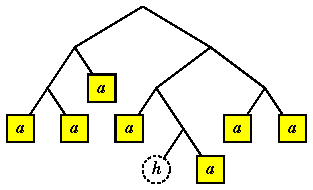
\includegraphics[width=1in]{deriv-tree}}

% Abstract
%
% Algebraic data types are central to typed functional programming,
% sitting at a happy intersection of theory and practice.  I will
% define and give examples of algebraic data types, and then go on to
% explain what is meant by the derivative of an algebraic data type.
% In the second part of the talk I will show how to constrain
% algebraic data types by a given regular expression, including
% finding derivatives a special case. No particular background is
% assumed; my goal is to convey not a particular result per se, but
% rather an appreciation for some of the beautiful overlap between
% algebra, combinatorics, calculus, and computer science.

%%%%%%%%%%%%%%%%%%%%%%%%%%%%%%%%%%%%%%%%%%%%%%%%%%%%%%%%%%%%

\begin{document}

\begin{xframe}{}
   \titlepage
\end{xframe}

\begin{xframe}
  \begin{center}
    Joint work with: \bigskip

    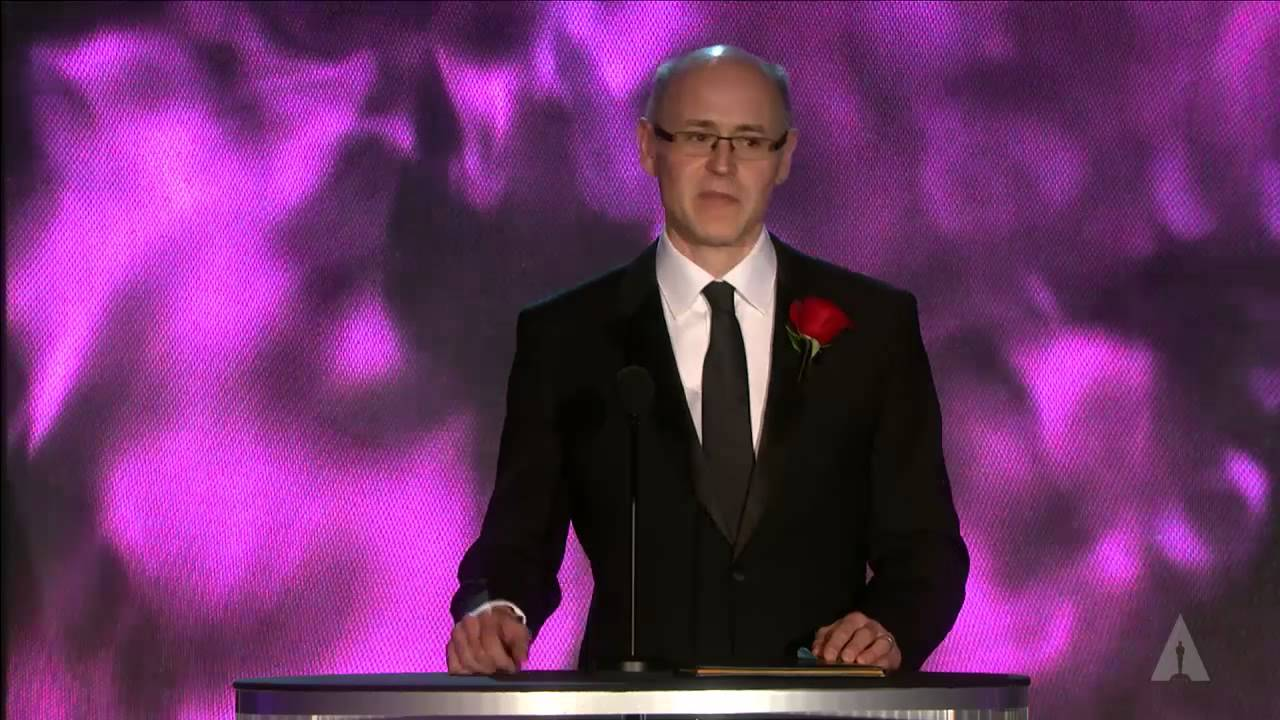
\includegraphics[width=3in]{dan} \\
    Dan Piponi
  \end{center}
\end{xframe}

\begin{xframe}
  %%% Fun to be here.  Work I do is at the intersection of math & CS.
%%% Please ask questions!  Part of my challenge is to translate some
%%% CS things for mathematicians and vice versa.

\begin{itemize}
\item Please ask questions!
\item Part I: get you to understand the title/problem statement
\item Part II: our solution (sketch)
\end{itemize}

%%% First two parts: get you to understand title, i.e. problem
%%% statement.  Part 3: our solution.  Based on joint work with Dan
%%% Piponi.

\end{xframe}

%% XXX section image: binary tree
%\def\sectionimg{dan.jpg}
\section{Polynomial functors}

\begin{xframe}{Polynomial functors}

  \begin{center}
  \[ F : \Set \to \Set \]
  elements $\to$ structures \bigskip

\begin{diagram}[width=200]
import           Data.List.Split
import           Diagrams

elts = map node [1,2,3,4::Int]
eltSet = atop (roundedRect 6 6 0.5)
       . centerXY
       . vsep 1 . map (hsep 1)
       . chunksOf 2
       $ elts    -- $

dia = [eltSet, arrowV (5 ^& 0), lsD] # map centerY # hsep 2 # frame 0.5
\end{diagram}
\bigskip

\onslide<2> aka \emph{algebraic data types}
  % think: \emph{(parameterized) combinatorial families}
  \end{center}
\end{xframe}

\begin{xframe}{Building polynomial functors}
  Polynomial functors are those $F : \Set \to \Set$ which can be built
  up out of:
  \begin{align*}
    0(A) &= \varnothing \\
    1(A) &= \{\star\} \\
    X(A) &= A \\
    (F + G)(A) &= F(A) \uplus G(A) \\
    (F \cdot G)(A) &= F(A) \times G(A)
  \end{align*}
\end{xframe}

\begin{xframe}{Example}
  \begin{gather*}
    1 + ((X \cdot X) + X) : \Set \to \Set \\
    (1 + ((X \cdot X) + X))(A) = \{\star\} \uplus ((A \times A) \uplus A)
  \end{gather*}
\end{xframe}

\begin{xframe}{Polynomial functor isomorphisms}
  Note that
  \begin{gather*}
    F + G \cong G + F \\
    F + (G + H) \cong (F + G) + H \\
    0 + F \cong F \cong F + 0 \\ \\
    F \cdot G \cong G \cdot F \\
    F \cdot (G \cdot H) \cong (F \cdot G) \cdot H \\
    1 \cdot F \cong F \cong F \cdot 1 \\ \\
    F \cdot (G + H) \cong F \cdot G + F \cdot H
  \end{gather*}
\end{xframe}

\begin{xframe}{Polynomial functor isomorphisms}
\[ 1 \cdot F \cong F \]

Example proof:

  \begin{align*}
    (1 \cdot F)(A) &= 1(A) \times F(A) \\
    &= \{\star\} \times F(A) \\
    &= \{(\star, f) \mid f \in F(A)\} \\
    &\cong F(A).
  \end{align*}
\end{xframe}

\begin{xframe}{Semirings}
  Up to isomorphism, polynomial functors form a (commutative) \emph{semiring}:

  \begin{itemize}
  \item Associative operations $+$, $\cdot$ with identities $0$, $1$
  \item $+$ is commutative
  \item $\cdot$ distributes over $+$
  \item $+$ does \emph{not} necessarily have inverses!
  \end{itemize}

  Other examples: $(\N,+,\cdot)$, $(\{\mathit{true},\mathit{false}\},
  \lor, \land)$, $(\R \union \{\infty\}, \max, +)$
\end{xframe}

\begin{xframe}{Implicit/recursive definition}
  We also allow mutually recursive definitions:
  \begin{align*}
    F_1 &= \Phi_1(F_1, \dots, F_n) \\
    &\vdots \\
    F_n &= \Phi_n(F_1, \dots, F_n)
  \end{align*}
\end{xframe}

\begin{xframe}{Example: lists}
  \[ L = 1 + X \cdot L \]

  \onslide<2->
  \[ L(A) = \{\star\} \uplus (A \times L(A)) \]
  \begin{center}
  \begin{tabular}{c m{3in}}
    $L(\N) =$ &
  \begin{diagram}[width=200]
    import           Diagrams

    dia = lsD # frame 0.5
  \end{diagram}
  \end{tabular}
  \end{center}
\end{xframe}

\begin{xframe}{Example: binary trees}
  \[ T = 1 + X \cdot T \cdot T \]

  \onslide<2->
  \[ T(A) = \{\star\} \uplus (A \times T(A) \times T(A)) \]
  \begin{center}
  \begin{tabular}{c m{3in}}
    $T(\N) =$ &
  \begin{diagram}[width=200]
    import           Diagrams.TwoD.Layout.Tree

    import           Diagrams

    dia = frame 0.5
        . hsep 3
        . (++ [ellipsis])
        . map (centerY . drawTree)
        $ trees  -- $
  \end{diagram}
  \end{tabular}
  \end{center}
\end{xframe}

\begin{xframe}{Example: binary trees}
  Polynomial functors can be \textbf{directly encoded} in programming
  languages with \textbf{algebraic data types} (Haskell, OCaml, SML,
  Scala, F\#):
  \[ T = 1 + X \cdot T \cdot T \]
  \[ T(A) = \{\star\} \uplus (A \times T(A) \times T(A)) \]
  \begin{verbatim}
       data T a = Empty | Node a (T a) (T a)
  \end{verbatim}
\end{xframe}

\begin{xframe}{Example: even/odd lists}
  \begin{align*}
    E &= 1 + X \cdot O \\
    O &= X \cdot E
  \end{align*}

  \begin{center}
  \begin{tabular}{c m{3in}}
    $E(\N) =$ &
  \begin{diagram}[width=200]
    import Diagrams
    dia = hsep 2 (map drawList [[], [3 :: Int,7], [3,7,2,8]] ++ [ellipsis])
        # frame 0.5
  \end{diagram}
  \\
  $O(\N) =$ &
  \begin{diagram}[width=150]
    import Diagrams
    dia = hsep 2 (map drawList [[3 :: Int], [3,7,2]] ++ [ellipsis])
        # frame 0.5
  \end{diagram}
  \end{tabular}
  \end{center}
\end{xframe}

\begin{xframe}{``Polynomial''?}
  All polynomial functors are isomorphic to \[ a_0 + a_1 X + a_2 X^2 +
  a_3 X^3 + \dots \] with $a_i \in \N$ ($n = 1 + \dots + 1$)
  \vspace{0.75in}

  % \begin{center}
  % {\small (mumble generating functions mumble blah \dots)}
  % \end{center}
\end{xframe}

%%% Do I need to say something about arbitrary arities?  OR can I just
%%% sweep that under the rug?

\begin{xframe}{``Functors''?}
  These are actually \emph{functors} $\Set \to \Set$: given a function
  we can apply it to every element in a structure (``map'').  E.g.:
  \[ T(x \mapsto x + 1) \]
  \begin{center}
  \begin{diagram}[width=200]
    import Diagrams
    dia =
      [ drawTree (trees !! 2)
      , arrowV (4 ^& 0)
      , drawTree (fmap succ (trees !! 2))
      ]
      # map centerY
      # hsep 2
      # frame 0.5
  \end{diagram}
  \end{center}
\end{xframe}

\begin{xframe}{Calculus!?}
  \begin{center}
  Analysis $\leftrightarrow$ Combinatorics \bigskip

  Example: \emph{differentiation}
  \end{center}
\end{xframe}

\begin{xframe}
  \begin{center}
    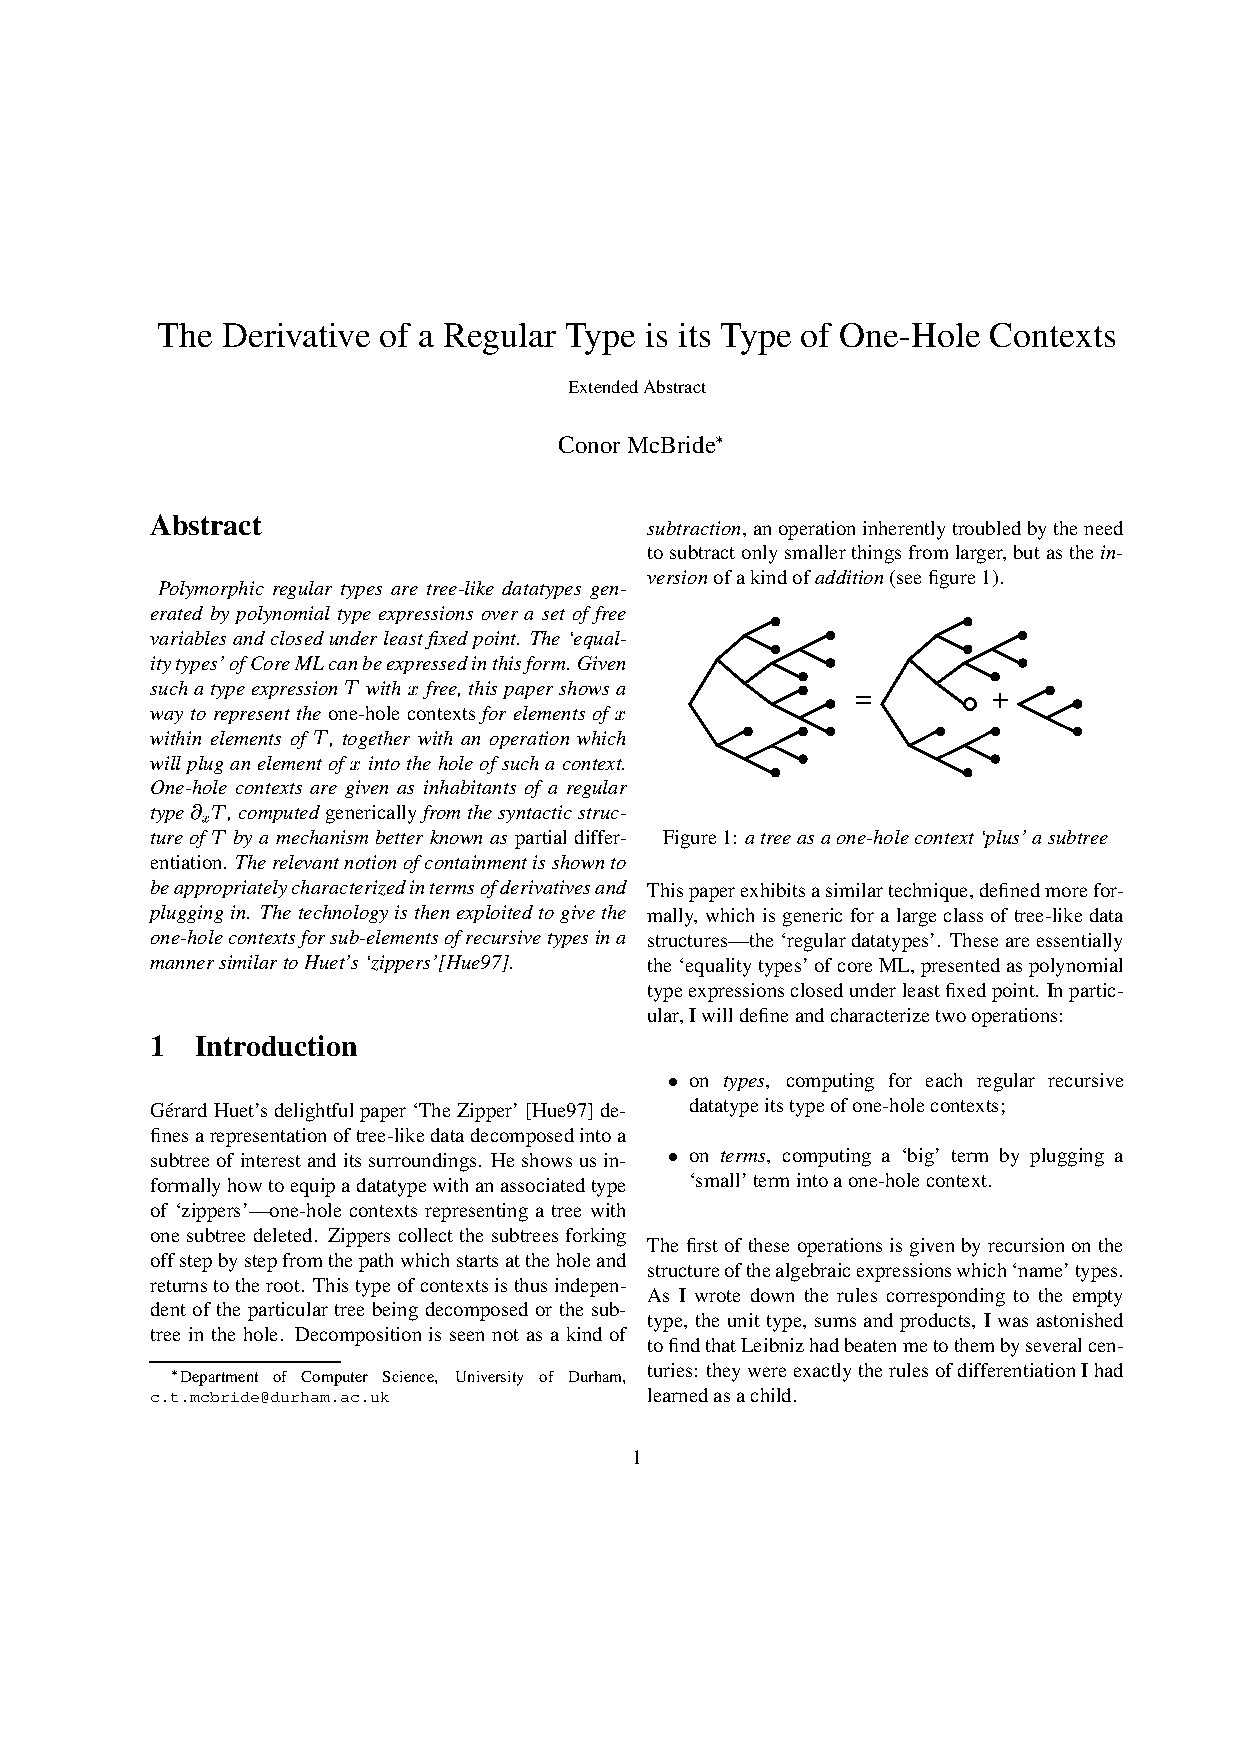
\includegraphics[width=3in]{diff-page1}
  \end{center}
\end{xframe}

\begin{xframe}
  \begin{center}
  \begin{tabular}{c m{1in} m{2in}}
    $T(\N)$ & trees of natural numbers, e.g. &
    \begin{diagram}[width=100]
      import Diagrams
      dia = drawTree (trees !! 3) # frame 0.5
    \end{diagram}
    \\
    $\displaystyle \left(\dd T X \right)(\N)$ &
    trees of natural numbers \emph{with a hole}, e.g. &
    \begin{diagram}[width=100]
      import Diagrams
      dia = drawNTree (poke 3 (trees !! 3)) # frame 0.5
    \end{diagram}
  \end{tabular}
  \end{center}
\end{xframe}

\begin{xframe}{Proof!}
\begin{itemize}
  \item Let $F$ be a polynomial functor.
  \item $\dd{F}{X}$ means what we would expect it to mean from calculus.
\end{itemize}
\bigskip

\onslide<2->
\emph{To show}: $\dd{F}{X}$-structures are (isomorphic to) $F$-structures with a
single $X$ replaced by a hole.

\begin{center}
\begin{diagram}[width=150]
  import Diagrams

  dia = hsep 1
    [ abstractTree "∂F"
    , text "≅"
    , abstractTree "F" # withHole
    ]
    # frame 0.5
\end{diagram}
\end{center}
\end{xframe}

\begin{xframe}{Proof!}
  \[ \dd{1}{X} \cong 0 \]
  \begin{center}
    $1$-structures have nowhere for a hole to go (they contain no
    data)
  \end{center}
  XXX picture?
\end{xframe}

\begin{xframe}
  \[ \dd{X}{X} \cong 1 \]
  \begin{center}
    An $X$-structure with a hole is just a hole.
  \end{center}
\end{xframe}

\begin{xframe}
  \[ \dd{(F+G)}{X} \cong \dd F X + \dd G X \]
  XXX picture and/or text
\end{xframe}

\begin{xframe}
  \[ \dd{(F \cdot G)}{X} \cong \dd F X \cdot G + F \cdot \dd G X \]

  \begin{center}
    XXX picture/text here
  \end{center}
\end{xframe}

\begin{xframe}
  \begin{itemize}
  \item Note this proof is also an \emph{algorithm} for computing $\dd
    T X$ from the definition of $T$. \bigskip
  \item These ``one-hole contexts'' turn out to be quite useful in the
    context of functional programming (``zippers''); the theory gives
    an automatic way to generate them.
  \end{itemize}

  \begin{center}
    \begin{diagram}[width=100]
      import Diagrams
      dia = drawNTree (poke 3 (trees !! 3)) # frame 0.5
    \end{diagram}
  \end{center}
\end{xframe}

% XXX if I have time.
%
% \begin{xframe}
%   \begin{align*}
%     T &= 1 + X \cdot T \cdot T \\
%     \dd T X &= 0 + T^2 + X \dd T X T + X T \dd T X \\
%   \end{align*}
%   %% picture: three kinds of trees with a hole
% \end{xframe}

% \begin{xframe}
%   \begin{align*}
%     \dd T X &= T^2 + X \dd T X T + X T \dd T X \\
%     &= T^2 + 2XT \dd T X
%     &= \mathsf{List}(2XT) \cdot T^2
%   \end{align*}
%   %% picture: chain of contexts etc.  Put this in if I have time.
% \end{xframe}

%% XXX section image: DFA
%% \def\sectionimg{dan.jpg}
\section{Regular expressions}

\begin{xframe}{Regular expressions}
  Regular expressions are a language of ``patterns'' for strings in
  $\Sigma^*$ (finite sequences of elements from ``alphabet'' $\Sigma$)

  \begin{align*}
    R &::= \varnothing && \text{never matches} \\
    &\mid \varepsilon && \text{empty string} \\
    &\mid a \in \Sigma && \text{``a''} \\
    &\mid R_1 \realt R_2 && \text{$R_1$ or $R_2$} \\
    &\mid R_1R_2 && \text{$R_1$ followed by $R_2$} \\
    &\mid R^* && \text{sequence of zero or more $R$}
  \end{align*}
\end{xframe}

\begin{xframe}{Examples}
  \begin{itemize}
  \item $a^*b^*$ \quad matches ``b'', ``aaa'', ``aaaabbb'', \dots
  \item $a^* b (c+d)$ \quad matches ``abd'', ``bd'', ``aaaabc'', \dots
  \item $((a+b)^*c)^*$ \quad matches ``aababcacaabbabc'', \dots
  \end{itemize}
\end{xframe}

\begin{xframe}{Constraining polynomial functors}
  \begin{itemize}
  \item Generalize to multivariate polynomial functors \[ F : \Set^n
    \to \Set \] i.e. $F(A_1, A_2, \dots, A_n)$
  \item Given a (univariate) $F$ and some regular expression $R$ over
    $\Sigma = \{A_1, \dots, A_n\}$
  \item Find a multivariate $F_R$ with the ``same shape'' as $F$ but
    whose sequences of elements come from a sequence of sets
    corresponding to $R$
  \end{itemize}
\end{xframe}

\begin{xframe}{Example}
     \begin{center}
       \[ L(A) = 1 + A \times L(A) \]
       \[ R = (AA)^* \]

  \begin{tabular}{c m{3in}}
  %   $L(\N) =$ &
  % \begin{diagram}[width=200]
  %   import           Diagrams

  %   dia = lsD # frame 0.5
  % \end{diagram}
  % \\
  $L_R(\N) =$ &
  \begin{diagram}[width=200]
    import           Diagrams

    ls2 = [[], [3,4 :: Int], [1,4,2,6], [3,9,2,0,8,4]]

    dia = vsep 1 (map drawList ls2) # frame 0.5
  \end{diagram}
  \end{tabular}
  \end{center}

\end{xframe}

\begin{xframe}{Example}
  \[ P = X + P^2 \]
  \[ R = a^*ha^* \]
  \begin{center}
    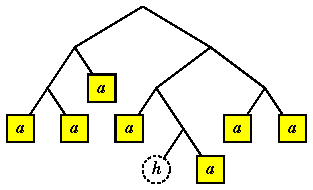
\includegraphics[width=2in]{deriv-tree}

    \onslide<2-> \dots this is just differentiation!
  \end{center}
\end{xframe}

\begin{xframe}{Example}
  \[ P = X + P^2 \]
  \[ R = b^*ha^* \]
  \begin{center}
    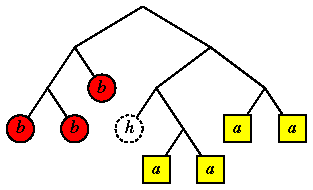
\includegraphics[width=2in]{dissect-tree}

  \onslide<2-> This is called a ``dissection'' and corresponds to
  \emph{divided difference}.
  \end{center}
\end{xframe}

\begin{xframe}{The problem}
  \begin{center}
  \textbf{Given a polynomial functor $F$ and regular expression $R$, compute
  a (system of mutually recursive, multivariate) polynomial functor(s)
  corresponding to $F$ constrained by $R$.}
  \end{center}
\end{xframe}

\section{The solution}

\begin{xframe}{DFAs}
  \begin{center}
    \textbf{D}eterministic \textbf{F}inite \textbf{A}utomata \bigskip

    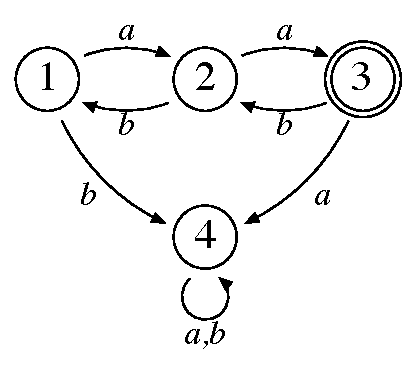
\includegraphics[width=2in]{example-DFA}

    DFAs = machines for identifying sequences
  \end{center}
\end{xframe}

\begin{xframe}{Punchline \#1}
  DFAs and regular expressions are ``about the same thing''! (Kleene,
  1951) \bigskip

  Every regular expression has a corresponding DFA (and vice versa).
\end{xframe}

\begin{xframe}{Example}
  \begin{center}
    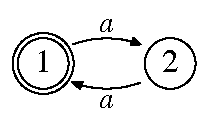
\includegraphics[width=2in]{even-DFA}

    \[ (aa)^* \]
  \end{center}
\end{xframe}

\begin{xframe}{Example}
  \begin{center}
    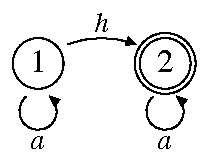
\includegraphics[width=2in]{deriv-DFA}

    \[ a^*ha^* \]
  \end{center}
\end{xframe}

\begin{xframe}{The setup}
  Given:
  \begin{itemize}
  \item Polynomial functor $F$
  \item DFA $D$
  \end{itemize} \medskip

  \onslide<2->
  Let $F_{ij}$ denote the (multivariate) polynomial functor
  \begin{itemize}
    \item with same shape as $F$
    \item constrained by sequences which take the DFA from state $i$
      to state $j$
  \end{itemize} \medskip

  \onslide<3->
  Ultimately we are interested in $\sum_{q \in \mathrm{final}(D)} F_{1q}$.
\end{xframe}

% XXX if time
% \begin{xframe}{Example}
%   XXX Show derivative DFA and all $T_{ij}$
% \end{xframe}

\begin{xframe}
  \begin{itemize}
  \item<+-> $0_{ij} = 0$
  \item<+-> $ 1_{ij} = \begin{cases} 1 \quad i = j \\ 0 \quad i \neq
      j \end{cases}$
  \item<+-> $X_{ij} = \text{(sum of) edge(s) from $i$ to $j$}$
  \item<+-> $(F + G)_{ij} = F_{ij} + G_{ij}$
  \item<+-> $(F \cdot G)_{ij} = \sum_{q \in \mathrm{states}(D)} F_{iq} G_{qj}$
  \end{itemize} \bigskip

  \onslide<6-> These are just the definitions of matrix operations!
\end{xframe}

\begin{xframe}
  %% XXX reword etc.
  \begin{center}
    This is a \emph{semiring homomorphism} from polynomial functors to
    $n \times n$ matrices of (arity-$|\Sigma|$) polynomial functors!
  \end{center}
\end{xframe}

\begin{xframe}{Example}
\[ L = 1 + XL, R = (aa)^* \]
\begin{center}
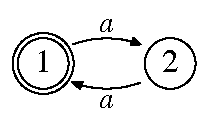
\includegraphics[width=1in]{even-DFA} \\
Transition matrix = $\begin{bmatrix}
  0 & a \\ a & 0
\end{bmatrix}$

\begin{multline*}
  \begin{bmatrix}
    L_{11} & L_{12} \\
    L_{21} & L_{22}
  \end{bmatrix}
  =
  \begin{bmatrix}
    1 & 0 \\
    0 & 1
  \end{bmatrix}
  +
  \begin{bmatrix}
    0 & a \\
    a & 0
  \end{bmatrix}
  \begin{bmatrix}
    L_{11} & L_{12} \\
    L_{21} & L_{22}
  \end{bmatrix}
  \\
  =
  \begin{bmatrix}
    1 + a L_{21} & a L_{22} \\
    a L_{11} & 1+ a L_{12}
  \end{bmatrix}.
\end{multline*}
\end{center}
\end{xframe}

\begin{xframe}
  \begin{center}
    Thank you! \bigskip

    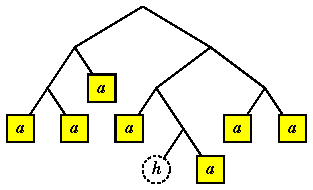
\includegraphics[width=1in]{deriv-tree}

    % XXX TODO include picture of publication first page
  \end{center}
\end{xframe}

% \begin{xframe}{Example}
%   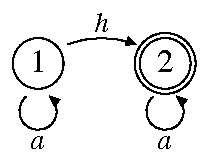
\includegraphics[width=2in]{deriv-DFA}

%   \[ a^*ha^* \]
% \end{xframe}

\end{document}